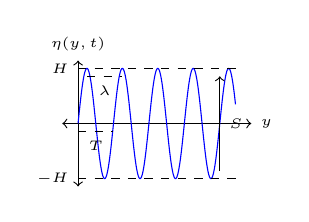
\begin{tikzpicture}[x=0.2cm, y=0.2cm,font=\tiny] % Adjusted scaling for smaller plot
    % Draw axes
    \draw[<->] (-1,0) -- (11,0) node[right] {$y$}; % Adjusted x-axis length
    \draw[<->] (0,-4) -- (0,4) node[above] {$\eta(y,t)$}; % Adjusted y-axis length
    % Draw wave
    \draw[blue, thin, domain=0:10, smooth,samples=900] plot (\x, {3.5*sin(8*pi*\x/9 r)});
    % Draw wave height
    \draw[dashed] (0,3.5) node[left] {$H$} -- (10,3.5) ; % Adjusted x-axis length
    \draw[dashed] (0,-3.5) node[left] {$-H$} -- (10,-3.5) ; % Adjusted x-axis length
    % Draw wave period
    \draw[dashed] (0,-0.5) -- (2.25,-0.5) node[midway, below] {$T$}; % Adjusted x-axis range
    
    % Draw wavelength
    \draw[dashed] (0.5625,3) -- (2.8125,3) node[midway, below] {$\lambda$}; % Adjusted x-axis range
    % Draw wave steepness
    \draw[->] (9,-3) -- (9,3) node[midway,right] {$S$}; % Adjusted x-axis range
\end{tikzpicture}


